\documentclass{standalone}

\usepackage{tikz}

% Four beetles -- A, B, C, and D -- occupy the corners of a square 10 inches along a side. A and C are male, B and C are female. Simultaneously A crawls directly towards B, B towards C, C towards D, and D towards A. If all four beetles crawl at the same constant rate, they will describe four congruent logarithmic spirals which meet at the centre of the square. How far does each beetle travel before they meet? The problem can be solved without calculus. 

\newcommand{\coorda}{10}
\newcommand{\coordw}{0}

\newcommand{\coordb}{0}
\newcommand{\coordx}{0}

\newcommand{\coordc}{0}
\newcommand{\coordy}{10}

\newcommand{\coordd}{10}
\newcommand{\coordz}{10}

\newcommand{\rate}{0.83}

\usepackage{xcolor}
% colours from latexcolor.com
\definecolor{amber}{rgb}{1.0, 0.75, 0.0}
\definecolor{bluegray}{rgb}{0.4, 0.6, 0.8}
\definecolor{amaranth}{rgb}{0.9, 0.17, 0.31}
\definecolor{asparagus}{rgb}{0.53, 0.66, 0.42}

\begin{document}
    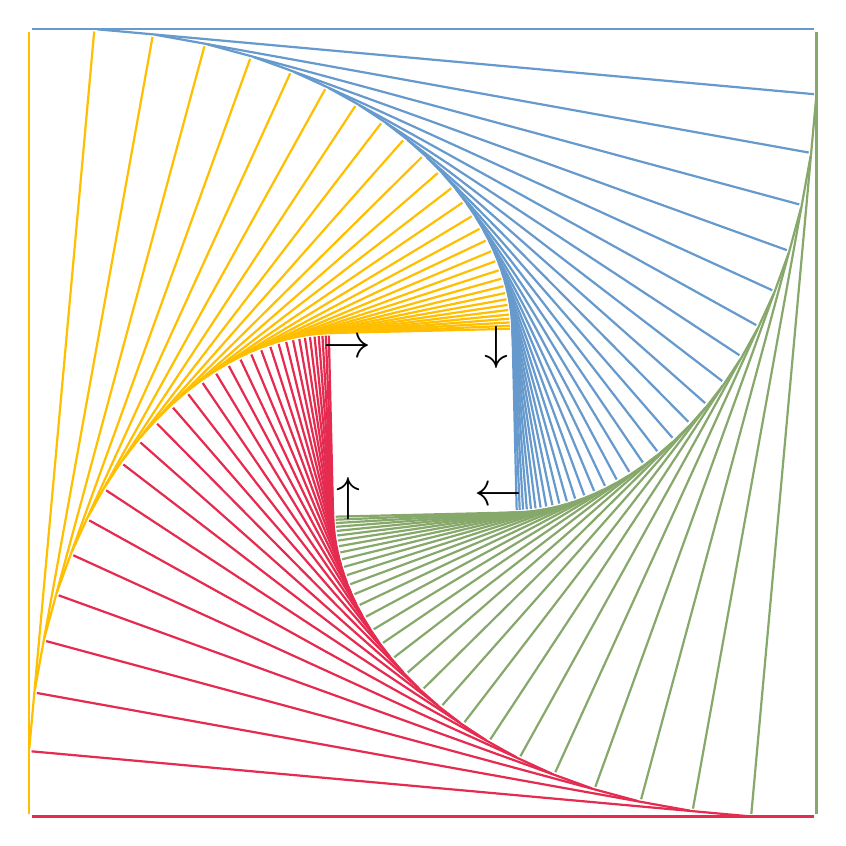
\begin{tikzpicture}[every path/.style={thick},every node/.style={inner sep=0}]
        
        
        \foreach \i in {0,...,30}{
            
            \node (A\i) at (\coorda,\coordw) {};
            \node (B\i) at (\coordb,\coordx) {};
            \node (C\i) at (\coordc,\coordy) {};
            \node (D\i) at (\coordd,\coordz) {};
            
            \draw[amaranth] (A\i) -- (B\i);
            \draw[amber] (B\i) -- (C\i);
            \draw[bluegray] (C\i) -- (D\i);
            \draw[asparagus] (D\i) -- (A\i);
            
            \pgfmathsetmacro{\angle}{atan((\coordx-\coordw)/(\coorda-\coordb))}
            \pgfmathsetmacro{\hdist}{\rate*cos(\angle)}
            \pgfmathsetmacro{\vdist}{\rate*sin(\angle)}
            
%            \node at (5,\i) {\angle,\hdist,\vdist};
            
            \pgfmathsetmacro{\newa}{\coorda-\hdist}
            \pgfmathsetmacro{\neww}{\coordw+\vdist}
            
            \pgfmathsetmacro{\newb}{\coordb+\vdist}
            \pgfmathsetmacro{\newx}{\coordx+\hdist}
            
            \pgfmathsetmacro{\newc}{\coordc+\hdist}
            \pgfmathsetmacro{\newy}{\coordy-\vdist}
            
            \pgfmathsetmacro{\newd}{\coordd-\vdist}
            \pgfmathsetmacro{\newz}{\coordz-\hdist}
            
            \pgfmathsetmacro{\newrate}{\rate*0.9}
            
            \global\let\coorda\newa
            \global\let\coordb\newb
            \global\let\coordc\newc
            \global\let\coordd\newd
            \global\let\coordw\neww
            \global\let\coordx\newx
            \global\let\coordy\newy
            \global\let\coordz\newz
            \global\let\rate\newrate
        }
        \node at (\coorda+0.2,\coordw+0.2) {\LARGE\(\uparrow\)}; % A
        \node at (\coordb+0.2,\coordx-0.2) {\LARGE\(\rightarrow\)}; % B
        \node at (\coordc-0.2,\coordy-0.2) {\LARGE\(\downarrow\)}; % C
        \node at (\coordd-0.2,\coordz+0.2) {\LARGE\(\leftarrow\)}; % D
        
    \end{tikzpicture}
\end{document}